\section{Electrode’s Kinetics}

We will now focus on the study of the kinetics of the electrochemical reactions happening on the electrodes boundaries. In particular, we will first start searching for a way to describe the transport of charge inside the system to then go into the mass transport phenomena. In this optics it will be quite useful to first recall some quantities that will be used inside the discussion.

Consider a general reduction reaction happening at an electrode, which can be written in the following form
\begin{equation}
    \ce{O + ne^-} \rightleftharpoons  \ce{R}.
\end{equation}
We will describe the rates at which a reaction take place by using the flux $\nu$ of electrons' moles that travels through the electrode surface. In this way we can describe also the current density on the surface by 
\begin{equation}
    J = nF\nu,
\end{equation}
where $n$ is the number of mole of electrons involved in the reduction reaction. Also, we know how both sides of the reaction are characterized by a transition rate $k_f$ and $k_b$ for the forward and backward direction, respectively. Such rates can be related to the flux easily by using the components surface density $C_i(x,t)$ and focus on the density at the surface as follows
\begin{align}
    &v_f = k_f C_O(0,t) = \frac{i_f}{nFA}, &v_b = k_b C_R(0,t) = \frac{i_b}{nFA},
\end{align}
where the surface was assumed to be at the position $x = 0$. If we connect this results we are already able to write down a form for the electrical current present in the system as
\begin{equation}
    \label{eq:TotalCurrentInterface}
    i = i_f - i_b = nFA[k_fC_O(0,t) - k_bC_R(0,t)].
\end{equation}
We only need to find a form for the quantities inside the equation, and that is basically what we are going to do in this section. 

Nevertheless, to be ready for that we shall also recall how we already know how $k$ can be computed by the use of transition state theory
\begin{equation}
    \label{eq:transitionRate}
    k = k_0\exp\left( -\frac{\Delta G^\ddagger}{RT} \right) = \kappa\frac{k_BT}{h}\exp\left( -\frac{\Delta G^\ddagger}{RT} \right).
\end{equation}
Where $\Delta G^\ddagger$ is the height of the barrier that separates the two states involved in the reaction, and the quantity $\kappa$ is called transmission coefficient expressing the probability to decay from the transition state to products.

\subsection{Butler-Volmer model}

To study the kinetics of electrons in the system we start from a standard condition of equilibrium in a one-electron single step reaction, which we approximate as in \figref{fig:ButlerVolmer}.
\begin{figure}[t]
    \centering
    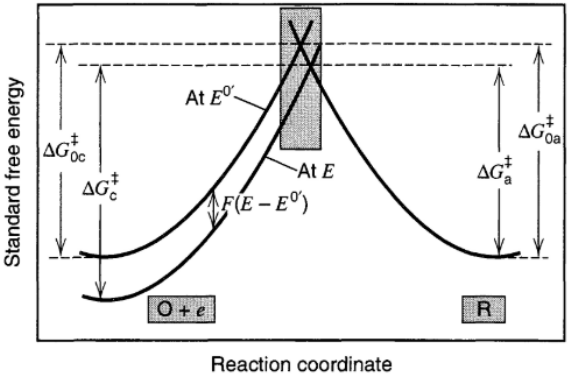
\includegraphics[width=0.45\textwidth]{Immagini/ButlerVolmer.png}
    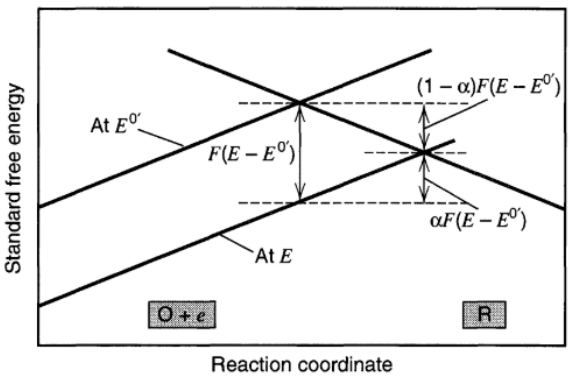
\includegraphics[width=0.45\textwidth]{Immagini/ButlerVolmer2.png}
    \caption{
        Approximation of the potential energy landscape inside a general reaction for some reaction coordinates. We are basically assuming that the reactants and products are minima in the energy and approximating the surrounding potential using second order Taylor expansion, so that the potential barrier is given by the interception of the parabolas.
    }
    \label{fig:ButlerVolmer}
\end{figure}
In that figure two conditions are depicted, a first one where we are in equilibrium so that the minima sits at the same height having so the same $\Delta G^\ddagger$ and therefore same rate, leading to $J = 0$. Then, we have the case where an external bias is applied and the energy of the electrons falls setting the reactants at lower potential generating a variation in the forward and backward barriers that can be estimated as follows
\begin{align*}
    &\Delta G_c^\ddagger = \Delta G_{0,c}^\ddagger - \alpha F(E - E^0), &\Delta G_a^\ddagger = \Delta G_{0,a}^\ddagger + (1 - \alpha) F(E - E^0).
\end{align*} 
Where $\alpha$ can be seen as an asymmetric factor, called transfer coefficient, that can range from zero to unity. Using these relations allows us to write down a form for the rates by inserting them inside \eqref{eq:transitionRate} to obtain
\begin{align}
    \label{eq:forwardRateC}
    &k_c = \kappa\frac{k_BT}{h}e^{-\frac{\Delta G^\ddagger_{0,c}}{RT}}\exp\left( -\frac{\alpha F(E-E^0)}{RT} \right), \\
    \label{eq:BackwardRateB}
    &k_a = \kappa\frac{k_BT}{h}e^{-\frac{\Delta G^\ddagger_{0,a}}{RT}}\exp\left( -\frac{(\alpha -1)F(E-E^0)}{RT} \right).
\end{align}
Knowing all of that we are able to obtain a really important result that is able to tell us the entity of the current inside our system as follows.
\thm{Butler-Volmer equation}
{
    The current flowing through the interface of an electrode, performing a general redox reaction, inside a well stirred solution is given by the equation
    \begin{equation}
        i = i_0\left[ e^{-\alpha\frac{F\eta}{RT}} - e^{-(\alpha - 1)\frac{F\eta}{RT}} \right].
    \end{equation}
    Where $i_0$ is the equilibrium current at the cathode and anode, while $\eta$ measure the bias applied as the difference between the cell potential and the standard one.
}
\pf{Proof}
{
    From \eqref{eq:forwardRateC} and \eqref{eq:BackwardRateB} we can see how, since the system was supposed to be in equilibrium without bias, meaning $E=E^0$, the rates have the properties of $k_c(E=0) = k_b(E=0)$. This brings us to write down that
    \begin{equation}
        k^0 = \kappa\frac{k_BT}{h}e^{-\frac{\Delta G^\ddagger_{0,c}}{RT}} = \kappa\frac{k_BT}{h}e^{-\frac{\Delta G^\ddagger_{0,a}}{RT}},
    \end{equation}
    which substituted back into the equation and inserted inside \eqref{eq:TotalCurrentInterface} gives the result
    \begin{equation}
        i = FAk^0\left[ C_O(0,t)e^{-\alpha\frac{F(E - E^0)}{RT}} - C_R(0,t)e^{-(\alpha - 1)\frac{F(E-E^0)}{RT}} \right].
    \end{equation}
    Now, in the equilibrium we have that $i = 0$ meaning how $i_c = i_a = i_0$ taking the name of \textbf{exchange current}, which can be found out easily from previous equation. In fact, by assuming equilibrium mass transfer is much faster than charge one surface concentration in electrode is equal to bulk one $C_0(0, t) = C_{O,b}$, so that we can write down
    \begin{equation}
        i_0  = FAk^0c_{O,b} e^{-\alpha\frac{F(E_{eq}-E^0)}{RT}}.
    \end{equation} 
    Since the system is at equilibrium we can use also Nernst equation in order to express the value of $E_{eq}$ as a function of concentration so that we can rewrite $i_0$ as
    \begin{align}
        &\frac{C_{O,b}}{C_{R,b}} = \exp\left[ \frac{F}{RT}(E_{eq} - E_0) \right], & i_0 = FAk^0 C_O^{1-\alpha}C_R^\alpha.
    \end{align}
    Inserting it inside the previous equation of $i$ and defining the \textbf{overpotential} $\eta$ as the difference $E - E_0$
    \begin{equation}
        i = i_0\left[ \frac{C_O(0, t)}{C_{O,b}} e^{-\alpha\frac{F\eta}{RT}} - \frac{C_O(0, t)}{C_{O,b}} e^{-(1-\alpha)\frac{F\eta}{RT}} \right],
    \end{equation}
    then in a stirred solution we also can assume that the surface concentration is equal to bulk one even out of equilibrium having that the fracions simplifies obtaining the right equation wanted.
}
\noindent
This equation is the key to understand how we can act on the variables of the system in order to boost the kinetics of the reaction. In particular, we can see how increasing both the external bias or the temperature can have huge effect on the reaction itself due to the exponential dependence. Also, one can see how the value of the exchange current posses a really important role since 
\begin{figure}[t]
    \centering
    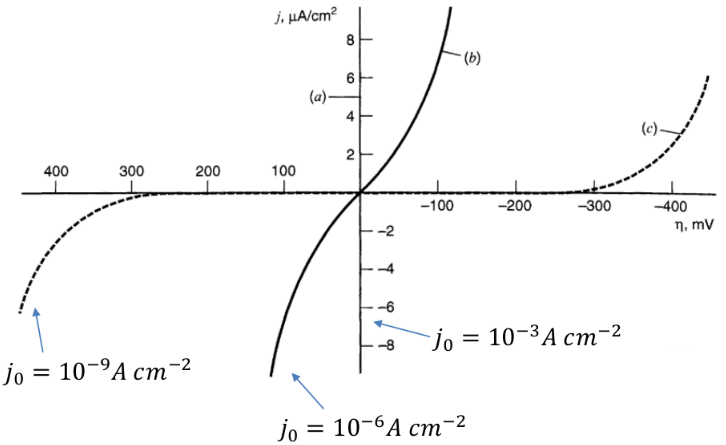
\includegraphics[width=0.8\textwidth]{Immagini/CurrentTrans.png}
    \caption{
        Graphic of the net current inside the cell as a function of the overpotential for different values of the exchange current, showing how the value of $i_0$ gives a great contribution to the overall current.
    }
    \label{eq:CurrentTrans}
\end{figure}
we can see from \figref{eq:CurrentTrans} how a lower $i_0$ gives a more \textbf{sluggish kinetics}. Where, a kinetics is more sluggish if you need a higher potential in order to obtain any net current at all inside the system.

Knowing such form for the current we can use it in order to perform some interesting computations regarding the kinetics properties. In particular, we can extract information about $\alpha$ and $i_0$ thanks to low and large $\eta$ regime. In the former case we have that a Taylor expansion leads us to the linear form
\begin{align}
    &i = -R_{ct}\eta, &R_{ct} = \frac{i_0 F}{RT},
\end{align}
the resistance $R_{ct}$ is called \textbf{charge-transfer resistance} and represent the impedance to charge transport intrinsic in the solution. Then, we can look at the case where $\eta \gg 1$, so that one of the two terms in the Butler-Volmer equation dominate so that we can easily write down
\begin{align}
    &i = i_0 e^{-\alpha \frac{F\eta}{RT}}, &\eta = \frac{RT}{\alpha F} \ln i_0 - \frac{RT}{\alpha F}\ln i.
\end{align}
Therefore, the potential linearly depends on the logarithm of the current giving rise to the form $\eta = a + b \ln i$ also called \textbf{Tafel theory}. The two constants inside such equation can be obtained with ease in experiments allowing us to estimate the values of both $\alpha$ and $i_0$.

\subsection{Mass transfer kinetics}

Butler-Volmer model allowed us to see how the kinetics of the system depends also on the surface concentration at the electrodes $C_i(0,t)$, which changes over time due to mass transport inside the material. Thus, we can't limit ourselves to the simple study of charge transport but to obtain a satisfying result we shall account also for the mechanisms of migration, convection and diffusion of material that can limit the flux of ions in the cell. In order to create such a model we are going to suppose to work in Nernstian conditions, so that equilibrium is present and the potential is given by Nernst equation, and we will also assume that the reaction is governed mass transport. Meaning that the rate at which the electroactive species is brought to the surface defines the current density
\begin{equation}
    J = nF\nu_{nt},
\end{equation}
where $\nu_{nt}$ is the flux of matter inside the electrolyte. Nevertheless, that is only the beginning of the model what we need to do now is to find out a more precise way to describe it.

The best way to model the flux of particle we can use a general form given by the sum of the contribution given by the three main processes mentioned before
\begin{equation}
    \nu_i(x) = -D_i\pdv{c_i}{x} - \frac{z_i F}{RT}D_i c_i\pdv{\Phi}{x} + c_iv(x).
\end{equation}
Where we have, in order, diffusion, migration and convection contribution, and $v$ represent the velocity of the solution in a certain point. Obviously such an equation is really complex, therefore we usually need to simplify it by setting ourselves in a situation where one or two contributions can be neglected such as:
\begin{itemize}[align=left, leftmargin=*]
    \item[\textbf{Diffusion.}] Introducing stirring;
    \item[\textbf{Migration.}] Addition of a concentrated supporting electrolyte;
    \item[\textbf{Convection.}] Avoiding vibrations or stirring. 
\end{itemize}
Therefore, we can choose to use one or more trick in order to eliminate the related processes. Thus, we are going to imagine to work in a diffusion limited process so that $\nu_i$ is defined simply by Fick's first law and the current density becomes
\begin{equation}
    J = nF\nu_d = nFD\eval{\dv{C_O}{x}}_{x=0}.
\end{equation} 
Where the derivative is evaluated at the interface and in a stirred solution we can assume that the bulk concentration is stable in the middle of the solution, meaning that $C_O$ is constant at $C_{O,b}$ for $x$ large enough. In this way we can approximate the derivative simply as a difference of the kind
\begin{equation}
    J \approx nFD\frac{C_{O,b} - C_{O}(x=0)}{\sigma},
\end{equation}
where $\sigma$ is a constant that needs to be tuned in order to optimize the approximation called \textbf{Nernst Diffusion Layer thickness} and can be seen in \figref{fig:ApproxDensGrad}.
\begin{figure}[t]
    \centering
    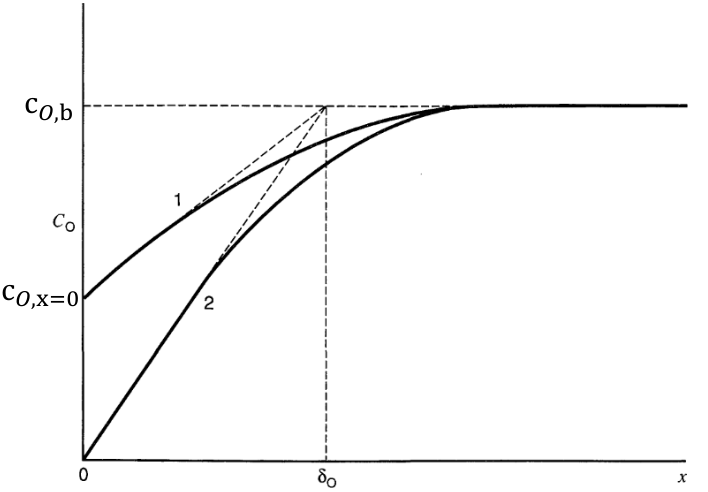
\includegraphics[width=0.8\textwidth]{Immagini/ApproxDensGrad.png}
    \caption{
        Representation of the concentration gradient approximation to understand what $\sigma$ effectively looks like and how the concentration is.
    }
    \label{fig:ApproxDensGrad}
\end{figure}
From that we can see how the diffusion is quicker the smaller $\sigma$ is or the more negative the potential becomes. Still, it's quite difficult to know the value of $\sigma$ so that it's value is usually combined with the diffusivity defining the \textbf{mass-transfer coefficient} $m_i = D_i/\sigma_i$.